 \documentclass{beamer}
%\documentclass[handout]{beamer}
\usetheme{metropolis}

%\setbeameroption{show notes}
%\setbeameroption{show notes on second screen}

% Packages
\usepackage[utf8]{inputenc}

\usepackage{animate}

\usepackage{appendixnumberbeamer}
\usepackage{xcolor}
\usepackage{multirow}
% Maths
\usepackage{amsthm}
\usepackage{tikz}
\usetikzlibrary{cd}

% Package Settings
% AMSTHM
\theoremstyle{plain}
\newtheorem{thm}{Theorem}[section]
\newtheorem{mylemma}[thm]{Lemma}
\newtheorem{cor}[thm]{Corollary}
\newtheorem{rem}[thm]{Remark}
\newtheorem{alg}[thm]{Algorithm}

\theoremstyle{definition}
\newtheorem{defn}[thm]{Definition}

\newcommand{\TODO}[1]{{\color{red}*** #1 ***}}

\input{./abbreviations.tex}

\title{Normalisatoren primitiver Gruppen mit nicht-regulären
Sockeln in polynomieller Zeit}
\date{July 10th, 2020}
\author{Sergio Siccha}
%\institute{Lehr- und Forschungsgebiet Algebra, RWTH Aachen}

\begin{document}

\maketitle
\note{
VERSION WITH NOTES!
}

\begin{frame}[standout]
\begin{itemize}
\item erklären
\begin{itemize}
\item Gruppe
\end{itemize}
\end{itemize}
\end{frame}


\begin{frame}[plain, noframenumbering]{Übersicht}
\begin{itemize}
\setlength{\itemsep}{\fill}
\item Warum?
\item Was?
\item Wie?
\end{itemize}
\end{frame}

\section{Motivation}
\begin{frame}{Gruppen (1)}
Warum Gruppen?

\pause
Gruppen
\begin{itemize}
\item sind nützlich
\pause
\item sind interessant
\end{itemize}
\end{frame}

\note{
Anwendungen
\begin{itemize}
\item Schwarze Löcher
\item Kryptographie (Verschlüsselung)
\item Versuchsdesign
\item $\ldots$
\end{itemize}
}

\begin{frame}{Gruppen (2)}
Gruppen beschreiben Symmetrien.
\\[-2em]
\begin{columns}
\begin{column}{0.4\textwidth}
Vier Eigenschaften
\begin{itemize}
\pause
\item Neutrales Element
\pause
\item Abgeschlossen
\vspace{3.2em}
\end{itemize}
\end{column}
\begin{column}{0.5\textwidth}
\begin{center}
  \animategraphics[]{9}{animation/}{1}{9}
\end{center}
\end{column}
\end{columns}
\vspace{1.4em}
\end{frame}

\begin{frame}[noframenumbering]{Gruppen (2)}
Gruppen beschreiben Symmetrien.
\\[-2em]
\begin{columns}
\begin{column}{0.4\textwidth}
Vier Eigenschaften
\begin{itemize}
\item Neutrales Element
\item Abgeschlossen
\pause
\item Invertierbar
\pause
\item Assoziativ
\end{itemize}
\end{column}
\begin{column}{0.5\textwidth}
\begin{center}
  \animategraphics[]{12}{animation/}{1}{17}
\end{center}
\end{column}
\end{columns}
\vspace{-2em}
Gruppe die aus Vertauschungen besteht:
\emph{Permutationsgruppe}.

\pause
\emph{Disclaimer:} hier nur endliche Gruppen und Mengen!
\end{frame}

\note{
Im Folgenden immer Permutationsgruppen.
}

\begin{frame}{Klassifikation einfacher Gruppen}
Was sind die kleinsten Bausteine\footnote{math.: einfache Gruppen} der Gruppen?

\TODO{Bild Periodensystem einfacher Gruppen. Von Kay Magaard?}

Wie kann ich Gruppen zerlegen und zusammensetzen?
\end{frame}

\note{
Klassifikation ist einer der Stützpfeiler 
}

\begin{frame}{Normalisatoren}
Normalisatoren%
\footnote{$G, M \leq K$.
Normalisator von $G$ in $M$ ist
$N_M(G) = 
\set{ m \in M ~|~ G ^ m = G }
$.
}:

\begin{itemize}
\item Werkzeuge um Gruppen zu verstehen
\pause
\item für beliebige Gruppen schwer zu berechnen
\pause
\item kein effizienter Algorithmus bekannt
\end{itemize}
\end{frame}

\begin{frame}{Experimente}
Untersuchung mithilfe von Computern
\begin{itemize}
\item Manche Fragen können einfach beantwortet werden $\ldots$
\item $\ldots$ andere hingegen nur mit großem Aufwand.
\end{itemize}
\end{frame}

\begin{frame}{Wie schwer?}
\TODO{Bild vom Langen Johann. Captions und footnotes!}
\note{Vergleich mit Hochhaus: wollen jemanden besuchen und kennen nur den
Nachnamen.
Szenario 1: Klingelschilder sind alphabetisch sortiert
Szenario 2: Klingelschilder sind nicht sortiert
Szenario 3: Klingelschilder sind nicht beschriftet

Berechnen von Normalisatoren bewegt sich zwischen Szenario 2 und 3, je nachdem
welche Gruppe man erwischt hat.

Source:
Bild: BR/Carlo Schindhelm
URL: https://www.br.de/radio/bayern2/sendungen/zeit-fuer-bayern/hochhaus-langer-johann-erlangen-100.html
Datum: 08.07.20
}
\end{frame}

\note{Überleitung:
Was macht man, wenn man ein großes Problem nicht lösen kann? Man sucht
sich ein einfacheres.
}

\begin{frame}{Primitive Gruppen}
Eine transitive Permutationsgruppe $G \leq \sym \Omega$ heißt
\emph{imprimitiv},
\pause
falls es eine nicht-triviale
$G$-invariante Partition von $\Omega$ gibt,
\pause
sonst \emph{primitiv}.

\pause
\TODO{Bild Eier}
\end{frame}

\note{
Wie lässt sich eine Permutationsgruppe zerlegen?

Kleinsten Bausteine der Permutationsgruppen sind primitive.
}

\section{Resultat}
\begin{frame}%{Resultat}
\begin{block}{Satz}
Sei \textcolor{blue}{$G = \gen X \leq \sym \Omega$ eine primitive Gruppe
mit nicht-regulärem Sockel}.
\pause
Dann kann ein
\textcolor{orange}{Erzeugendensystem von $N_{\sym \Omega}(G)$}
\pause
in
\textcolor{green}{Zeit polynomiell beschränkt in $\abs X$ und $\abs
\Omega$} bestimmt werden.
\end{block}
\end{frame}

\note{
Erwähnen?:
Hoffnung:
bessere Algorithmen für "zusammengesetzte" Gruppen.
}

\section{Strategie}
\note{Struktur primitiver Gruppen ausnutzen}
\begin{frame}{Permutationsisomorphie}
\begin{block}{Notation}
\begin{itemize}
\item
$\Omega$, $\Delta$ bezeichnen Mengen
\item
$\sym \Omega$:
Gruppe aller Permutationen von $\Omega$
\item
$\alpha ^ g := g(\alpha)$
\end{itemize}
\end{block}

Zwei Gruppen $G \leq \sym \Omega$ und $H \leq \sym \Delta$ heißen
\emph{permutationsisomorph}, wenn
Isomorphismen $f : \Omega \to \Delta$ und $\phi : G \to H$ existieren,
sodass
$\forall g \in G, \omega \in \Omega$:
\[
    f( \omega ^ g ) = f(\omega) ^ {\phi(g)}.
\]
\end{frame}

\begin{frame}{Struktursatz primitiver Gruppen}
Der \emph{Sockel} einer Gruppe $G$, geschrieben
$\soc G$, ist das Erzeugnis aller minimalen Normalteiler.

Der Sockel einer primitiven Gruppe ist charakteristisch einfach.

\begin{block}{Satz von O'Nan-Scott}
Sei $G \leq \sym \Omega$ eine primitive Permutationsgruppe.
Bis auf Permutationsisomorphie kennen wir
\begin{itemize}
\item $\soc G$,
\item $N_{\sym \Omega}( \soc G )$.
\end{itemize}
\end{block}
\end{frame}

\note{
Sockel charakteristisch einfach $\Rightarrow$ Rekursion zu einfachen
Gruppen

Außerdem:
$N(\soc G)$ enthält $N(G)$.
Index von $G$ in $N(\soc G)$ ist winzig.
$N(\soc G)$ entsteht durch Produktop. Kranzprodukte.
}

\begin{frame}{Strategie}
Sei $G \leq \sym \Omega$ eine primitive Permutationsgruppe.

Sei $M := N_{\sym \Omega}(\soc G)$.
Es gilt $N_{\sym \Omega}(G) = N_M(G)$.

Bestimme
\begin{itemize}
\item $M := N_{\sym \Omega}(\soc G)$.
\item Gruppenhom.
$
    \rho : M \to S_k
$
mit $k \in O(\log \abs \Omega)$
und
\[
    N_{\sym \Omega}(G) = N_{M}(G) = \rho ^ {-1}( N_{\rho(M)}(\rho(G)) ).
\]
\end{itemize}
\end{frame}

\note{
Log. Reduktion einfach. Dann im Endeffekt nur Algorithmus von Daniel Wiebking.

Normalisator des Sockels mehr Aufwand.
}

\begin{frame}{Logarithmische Reduktion}
Kranzprodukt in Produktoperation
$\rightarrow$
imprimitive Operation

\pause
Sockel herausfaktorisieren
\end{frame}

\note{
Produkt $\rightarrow$ imprimitiv macht $d ^ \ell$ zu $d \cdot \ell$ Punkten.

Kranzprodukt:
\begin{itemize}
\item Symmetrische Gruppe auf Anzahl Komponenten von $\Omega ^ {\ast}$.
\item Sockel einfache Gruppen + äußere Automorphismen.
Nach herausfaktorisieren des Sockels bleiben nur die äußeren Automorphismen.
\end{itemize}



Wichtig:
$\log ^ 2(n)$ würde nur quasipolynomiellen Algorithmus liefern.
}


\section{Begriffe}
\begin{frame}
Frames:
\begin{itemize}
\item Gruppe
\item Normalisator
\item Primitiv
\end{itemize}
\end{frame}

\begin{frame}{Gruppen}
Eine Symmetrie kommt selten allein.

Vier Axiome:
\begin{itemize}
\item Abgeschlossen
\item Einheit
\item Assoziativ (verhält sich wie funktionen)
\item Inverse
\end{itemize}
\end{frame}

\begin{frame}{Gruppen: Beispiel}
Symmetrien eines Quadrats

Animation
\end{frame}

\begin{frame}{Permutationen}
Permutationen

Symmetrische Gruppe (viele Permutationen)
\end{frame}

\begin{frame}{Normalisatoren}
100 $\cdot$ \emph{Anzahl Atome in der Sonne} $\Rightarrow$ 7
\end{frame}


\section{Werkzeuge}
\note{
Perm-iso in kanonische Gestalt rekonstruieren.
Dann Klassifikation endlicher einfacher Gruppen anwenden.
}

\note{
Typ PA: einfachster nicht-trivialer Fall.
}

\begin{frame}{PA Typ}
Sei $G \leq \sym \Omega$ eine primitive Gruppe.
Dann ist $G$ vom \emph{Typ PA}, falls
eine einfache Gruppe
$T \leq \sym \Delta$
und ein Permutationsiso-
morphismus $(f : \Omega \to \Delta ^ \ell,~ \phi : G \to H)$ existieren
mit
\[
\phi (\soc G) = T ^ \ell \leq \sym(\Delta ^ \ell).
\]

\pause
\begin{block}{Korollar}
$G \leq \sym(\Delta ^ \ell)$ primitiv mit
$\soc G = T ^ \ell$.
Dann ist
\[
    N_{\sym (\Delta ^ \ell)}(\soc G) =
    N_{\sym \Delta}(T) \wr S_\ell.
\]
\end{block}
\end{frame}

\begin{frame}{Schwach kanonische Form - Typ PA}
Sei $G \leq \sym(\Delta ^ \ell)$ eine primitive Gruppe vom Typ PA.
\pause
Dann ist $G$ in \emph{schwach kanonischer Form}, falls
eine einfache Gruppe
$T \leq \sym \Delta$
existiert mit
\[
\soc G = T ^ \ell.
\]
\end{frame}


\begin{frame}{Schwach kanonische Form}
\begin{block}{Satz}
Sei $G \leq \sym \Omega$ eine primitive Gruppe. Ein Permutationsiso. in schwach
kanonische Form kann in polynomieller Zeit berechnet werden.
\end{block}

\pause
\begin{block}{Satz}
Sei $G \leq \sym \Omega$ eine primitive Gruppe in schwach kanonischer Form.
Dann kann $N_{\sym (\Omega)}(\soc G)$
in polynomieller Zeit berechnet werden.
\end{block}
\end{frame}

\note{das Beste zum Schluss.
Jeder der mal was mit Permutationsgruppen zu tun hatte, weiß, dass diese
schnell "messy" werden können.
Um WCF zu berechnen benutzen wir perm mors.


Motivation:
1. Für PA Typ: Wir schreiben $\soc G$ als \emph{Produkt} in einer geeigneten
Kategorie.

2. Ein Permutationsiso ist eindeutig durch die Gruppe $G$ und die
Punktabbildung $f : \Omega \to \Delta$ gegeben.

Also sollte es ausreichen $\Omega$ in $\Delta ^ \ell$ zu zerlegen.}

\begin{frame}{Morphismen von Permutationsgruppen}

Seien $f : \Omega \to \Delta$ und $\phi : G \to H$.
Ein Paar $F = (f, \phi)$ heißt
\emph{Permutationsmorphismus von $G$ nach $H$},
falls
$\forall g \in G, \omega \in \Omega$:
\[
    f( \omega ^ g ) = f(\omega) ^ {\phi(g)}.
\]

\pause
\begin{block}{Satz}
Permutationsgruppen zusammen mit Permutationsmorphismen und komponentenweiser
Verknüpfung bilden eine Kategorie $\mathbf{PermGrp}$.
\end{block}
\end{frame}

\note{
So berechnet man also Normalisatoren. :-)
}

\begin{frame}[standout]
Danke!
\end{frame}

\note{
Abschließende Worte?
Wie zurück vom Detaillierten zum großen Ganzen?
}

\appendix
\begin{frame}{Permutationsmorphismen: Produkte (1)}
\begin{block}{Satz}
$\mathbf{PermGrp}$ enthält alle endlichen Produkte.
\end{block}
\end{frame}

\begin{frame}{Permutationsmorphismen: Produkte (2)}
\begin{block}{Beispiel}
$\Omega := \set{1, \ldots, 4}$ und
$V := \langle a := (1,2)(3,4),~$%
$b := (1,3)(2,4) \rangle$.

\begin{figure}[H]
\centering
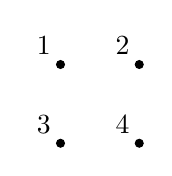
\begin{tikzpicture}
    % nodes
    \foreach \x in {1, ..., 2}
        \foreach \y in {1, ..., 2}
            \draw [fill] (\x, \y) circle [radius=0.050];
    \node [above left] at (1, 2) {{$1$}};
    \node [above left] at (2, 2) {{$2$}};
    \node [above left] at (1, 1) {{$3$}};
    \node [above left] at (2, 1) {{$4$}};
\end{tikzpicture}
\end{figure}

Ferner sei
$P_1 := (p_1, \pi_1)$ mit
\begin{align*}
p_1 &: \Omega \to \set{1,3},~~
1,2 \mapsto 1, ~~ 3,4 \mapsto 3,
\\
\pi_1 &: G \to \gen{(1,3)},~~
\id_\Omega, a \mapsto \id_{\set{1,3}},
~~b, ab \mapsto (1,3).
\end{align*}

Analog $P_2$.
Dann $P_1 \times P_2 : V \iso \gen{(1,3)} \times \gen{(1,2)}$
\end{block}
\end{frame}

\begin{frame}{Permutationsmorphismen: Produkte (3)}
\begin{block}{Satz}
Sei $G \leq \sym \Omega$.
Für $i = 1, \ldots, \ell$
seien
$(p_i : \Omega \to \Omega_i)$
mit $G$ kompatible Abbildungen,
\pause
die mit $\Omega$ ein Produkt in
$\mathbf{Set}$ bilden.
\pause
Ferner seien
$P_i = (p_i, \pi_i)$ die eindeutigen ``Fortsetzungen'' der $p_i$ zu
Permutationsepimorphismen
von $G$.
\pause
Dann gilt
\[
G \text{ bildet mit } (P_i)_{i \leq \ell} \text{ ein Produkt }
\iff
\prod \pi_i \text{ ist Epim. }
\]
\end{block}
\end{frame}


\begin{frame}{animation test 1}
\begin{center}
  \animategraphics[]{9}{animation/}{1}{9}
\end{center}
\end{frame}


\begin{frame}{animation test 2}
\begin{center}
  \animategraphics[]{12}{animation/}{1}{17}
\end{center}
\end{frame}

\end{document}
